\documentclass[12pt]{article}
\setlength{\arrayrulewidth}{0.5mm}
\setlength{\tabcolsep}{18pt}
\renewcommand{\arraystretch}{1.5}
\usepackage{tabularx}
\usepackage{adjustbox}
\usepackage{multirow}
\usepackage{tocloft}
\usepackage{tikz}

\usepackage[sorting=none]{biblatex}
\addbibresource{ref.bib}
\renewcommand\cftsecfont{\Large\bfseries}
\renewcommand\cftsecpagefont{\Large\bfseries}
\renewcommand\cftsubsecfont{\large\bfseries}
\renewcommand\cftsubsecpagefont{\Large\bfseries}
\usepackage[table,xcdraw]{xcolor}
\linespread{1}
% \usepackage[showframe]{geometry}
\usepackage{layout}
\usepackage{booktabs}
\usepackage{varwidth}
\usepackage[left=.75in, right=.75in, bottom=.5in, top=1in]{geometry}
\usepackage{ragged2e}
\usepackage{graphicx} % Required for inserting images
\usepackage{listings}
\usepackage{float}
\usepackage{verbatim}
\usepackage{color}
\definecolor{dkgreen}{rgb}{0,0.6,0}
\definecolor{gray}{rgb}{0.5,0.5,0.5}
\definecolor{mauve}{rgb}{0.58,0,0.82}

\lstset{frame=tb,
  language=Python,
  aboveskip=3mm,
  belowskip=3mm,
  showstringspaces=false,
  columns=flexible,
  basicstyle={\small\ttfamily},
  numbers=none,
  numberstyle=\tiny\color{gray},
  keywordstyle=\color{blue},
  commentstyle=\color{dkgreen},
  stringstyle=\color{mauve},
  breaklines=true,
  breakatwhitespace=true,
  tabsize=3
}
\graphicspath{{./logo/}}
\setlength{\voffset}{-.25in}
\setlength{\textheight}{650pt}
% \setlength{\textwidth}{470pt}
% \setlength{\oddsidemargin}{0pt}
\setlength{\topmargin}{0pt}
% \setlength{\marginparsep}{0pt}
% \setlength{\hoffset}{0in}
\setlength{\marginparwidth}{1in}
\setlength{\headsep}{5pt}
\title{\Huge \textbf{AI-Driven Stock Price Forecasting}\vspace{-2em}}
\date{\LARGE July 2023}











\begin{document}
\maketitle
{\centering{\huge{\textbf{CS F407: Artificial Intelligence}}}\par}
\vspace{0.25in}
\thispagestyle{empty}
\begin{center}
    
\includegraphics[scale=1]{logo/bits-logo.pdf}\\
\end{center}
\vspace{0.25in}
{\centering \LARGE{Under the supervision of\\ \textbf{Dr. Aneesh Chivukula}}\par}
\vspace{.1in}
{\centering
\begin{table}[b]
    {\centering \LARGE
    \begin{tabular}{|c|c|} \hline \centering
        \textbf{Group Members} & \textbf{ID}\\\hline
        Arya V Singalwar& 2020B3A71861H \\\hline
        M Varun Srinivas  & 2020B3AA0497H\\
        \hline \centering
        P Sai Shruthi & 2020B3A70904H\\
        \hline
    \end{tabular}\par}
\end{table}\par}
\pagebreak

\begin{center}
    \section*{\LARGE Abstract}
\end{center}
“AI-Driven Stock Price Forecasting” presents a comprehensive method for predicting Bajaj Finserv's stock price for the next 30 days, leveraging the previous ten years of closing prices. This model aids in managing risks and optimizing investment strategies for portfolio managers, risk management experts, financial regulators, and traders. The employed predictive models include Stacked Long Short-Term Memory (LSTM), Extreme Gradient Boosting (XGBoost), and Facebook's Prophet Model, known for their efficiency in stock price prediction.

The dataset includes daily opening, high, low, closing, adjusted closing prices, and volume of Bajaj Finserv shares. Data preprocessing steps like scaling, handling missing values, and reshaping for LSTM were undertaken to improve model performance.

LSTM, a recurrent neural network, was employed due to its aptness in forecasting sequence or time-series data. The LSTM model was built with three LSTM layers and a final dense layer configured for specific requirements0.

The Prophet model, a forecasting tool by Facebook, follows a piecewise linear or logistic growth curve trending additive regression model. It considers the seasonal component in predictions, ensuring greater accuracy.

XGBoost model, an efficient machine learning method, was employed for its unique tree pruning strategy, handling of sparse data and missing values, and in-built cross-validation at each iteration of the boosting process. 

Performance assessment employed metrics like RMSE and MAPE. FBProphet Model outperformed the other models. Models were tested for unseen data and future predictions, proving effective for making informed investment decisions. Despite the limitations, these models delivered promising results and are valuable tools for predicting stock prices.

\thispagestyle{empty}
%Abstract goes here
\pagebreak
\Huge{\textbf{Contents}}
\vspace{.1in}
    \hrule height 0.25mm
\vspace{0.15in}
\tableofcontents
\thispagestyle{empty}
\pagebreak
\clearpage
\pagenumbering{arabic}
\section{Introduction}
\normalsize{Predicting stock prices is a task that has attracted the attention of numerous researchers and investors. Accurately predicting the stock price of companies like Bajaj Finserv carries great significance for investors, traders, and financial regulators. 

The stock market is a complex system influenced by various factors, including economic indicators, geopolitical events, and company specific news. Therefore predicting stock prices requires a thorough analysis of these factors. This project aims to predict the stock price of Bajaj Finserv for the next 30 days using data from its previous 10 year closing prices. The potential implications of this predictive model are extensive. 

It can be a valuable tool for portfolio managers. Risk management experts, and financial regulators alike. Portfolio managers can optimize their investment strategy and maximize returns by utilizing the predicted stock prices. 

Risk management experts can effectively manage and mitigate investment risks based on these predictions. Financial regulators can monitor the stability of the financial system using this model and identify potential threats to the market. Even ordinary investors and traders can benefit from this predictive model by making informed decisions about buying and selling stocks to minimize risks while maximizing returns

Stacked LSTMs, XGBoost, and Facebook's Prophet Model will be utilised in this project to predict the stock price of Bajaj Finserv. These models were selected because they are often used in the field of stock price prediction and have demonstrated promising outcomes in prior studies.

The ability to forecast the price of Bajaj Finserv's shares has important ramifications for traders, portfolio managers, risk management specialists, and financial regulators. These stakeholders can maximise their returns and reduce their risks by making well-informed decisions that can affect the stock price. Advanced predictive models, such Stacked LSTMs, XGBoost, and Facebook's Prophet Model, can serve to offer insightful information and boost the precision of stock price forecasts.
}
\section{Data Preprocessing}
\vspace{0in}
\normalsize{The dataset used was obtained from the National Stock Exchange of India (NSE) \cite{nseindia}. The dataset contains 10-year data on the stock of Bajaj Finserv Ltd.} 
\subsection{Data Understanding}

\normalsize{The data begins on 2012-11-11 and continuing until the date cut off, each row in this table represents a separate trading day. The columns include the date, the opening price ("Open"), the highest price the stock reached that day ("High"), the lowest price it reached ("Low"), the closing price at the end of the trading day ("Close"), the adjusted closing price ("Adj Close") which takes into account things like dividends and stock splits, and the volume of shares traded that day ("Volume"). The numbers "null" displayed in the first row indicate that there is missing data for that particular day. As a result of this, we need to cleanse the data to make accurate predictions using the data in the future. This data may be analyzed to discover various patterns, trends, and insights, such as the general price trend over time, variations in volume, or daily price volatility. }
\subsection{Data Preparation}
\begin{enumerate}
    \item The values in the dataset needed to be scaled down between 0 and 1, as the range of stock price is varying for the 10 years.
    \item  Data was then split into training and testing datasets, where the training data size was 65\% and the testing data size was 35\%. 
    \item A time-step of 100 days was taken initially to create the training and testing data.
    \item In order to use the data for the stacked LSTMs, the data was reshaped into 3 dimensions - [samples, time steps, features]
\end{enumerate}



\section{Model Development}
\normalsize{In total, 3 different models were developed with the same goal of forecasting the price of BAJAJFINSV stock for the next 30 days. All the models followed the same data preparation approach for generating training and testing datsets. The models differ in terms of their architecture and as a result, in terms of their accuracy.}
\\
\subsection{Long Short-Term Memory ($LSTM$) Model}
Stacked $LSTMs$ were created by importing it from the $TensorFlow$ library. We fit the data and run 100 epochs initially, and check RMSE after using Adam optimiser. The function for calculating \textbf{MAPE} was added to evaluate the performance of the model.

The design incorporates a specific type of recurrent neural network known as long short-term memory (LSTM), which is well-suited for forecasting sequences or time series data. It utilizes three LSTM layers and a final dense layer. The LSTM layers retain information from past inputs, making them effective for tasks such as natural language processing and stock price forecasting. The model's architecture includes a sequence-returning LSTM layer followed by another sequence-returning LSTM layer, and a third LSTM layer that provides a single output. The dense layer with a single unit predicts the closing price of the stock. The model is trained using the Adam optimizer and mean squared error loss function. Performance evaluation is conducted using metrics like RMSE and MAPE. The trained LSTM model is used to forecast future closing prices based on unseen test data, using the last 100 days to predict the subsequent 30 days. Matplotlib is employed for visualization. While LSTM models excel in time series prediction, they require careful hyperparameter selection and can be computationally expensive. Nonetheless, they prove effective for problems with longer data dependencies.

Overall, the design incorporates an LSTM model with its specific architecture and utilizes it for time series forecasting. It demonstrates the model's training process, evaluation metrics, and its application to forecast future closing prices. The limitations of LSTM models are highlighted, emphasizing the need for careful hyperparameter selection and the computational complexity involved. Despite these challenges, LSTM models are found to be effective for time series prediction problems with longer data dependencies.
\pagebreak

Here is the code for the model:
\begin{center}
    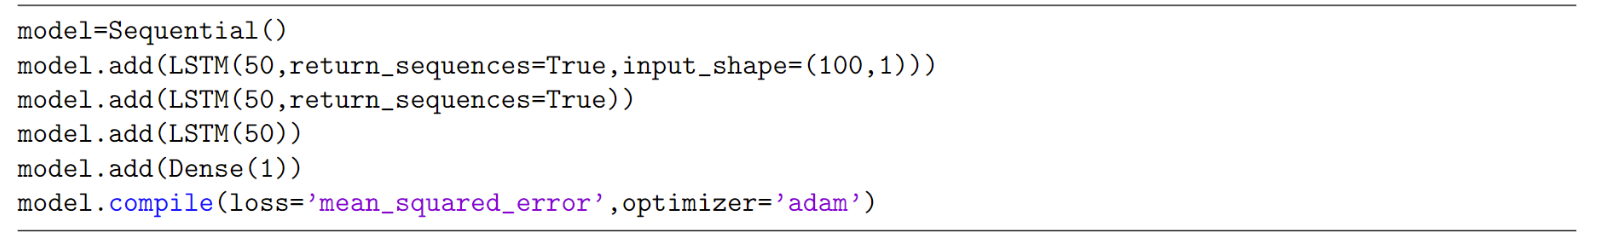
\includegraphics[scale=0.59]{codes/code 1.png}
\end{center}
% \begin{lstlisting}
% model=Sequential()
% model.add(LSTM(50,return_sequences=True,input_shape=(100,1)))
% model.add(LSTM(50,return_sequences=True))
% model.add(LSTM(50))
% model.add(Dense(1))
% model.compile(loss='mean_squared_error',optimizer='adam')
% \end{lstlisting}
The model summary can be seen as-
\begin{center}
    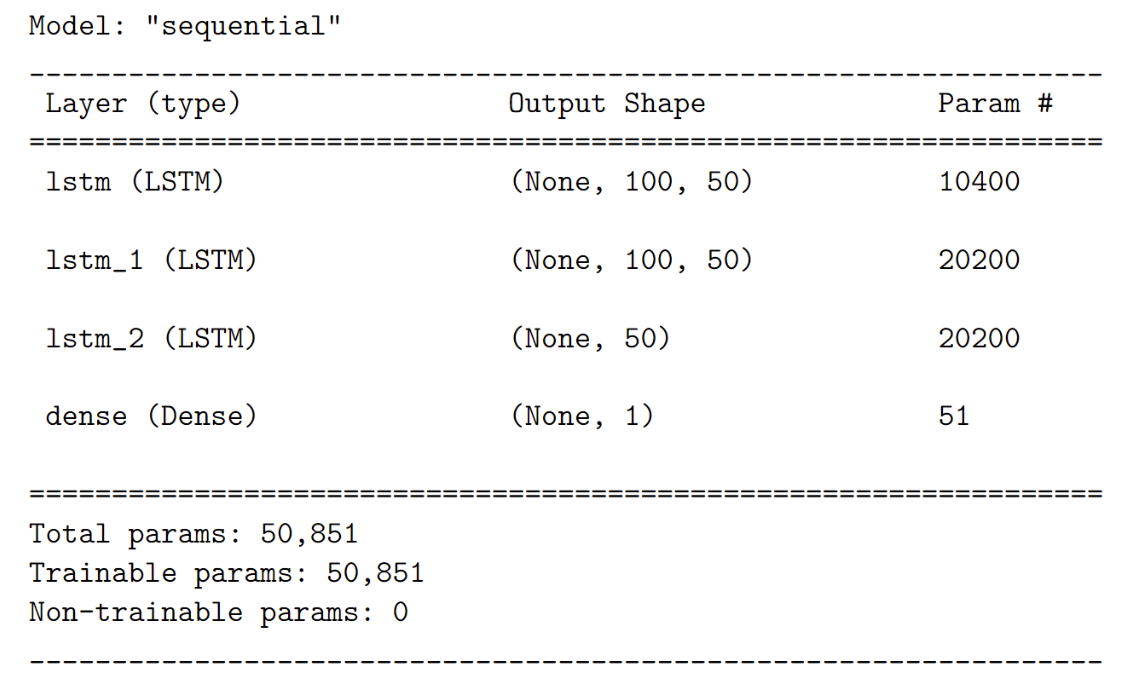
\includegraphics[scale=0.5]{codes/code 2.png}
\end{center}
% \begin{center}
% \begin{varwidth}{\linewidth}
% \begin{verbatim}
% Model: "sequential"
% _________________________________________________________________
%  Layer (type)                Output Shape              Param #   
% =================================================================
%  lstm (LSTM)                 (None, 100, 50)           10400     
                                                                 
%  lstm_1 (LSTM)               (None, 100, 50)           20200     
                                                                 
%  lstm_2 (LSTM)               (None, 50)                20200     
                                                                 
%  dense (Dense)               (None, 1)                 51        
                                                                 
% =================================================================
% Total params: 50,851
% Trainable params: 50,851
% Non-trainable params: 0
% _________________________________________________________________
% \end{verbatim}
% \end{varwidth}
% \end{center}
The train-test fit for stacked LSTM Model can be seen in the following figure- 
\begin{figure}[H]
    {\centering
    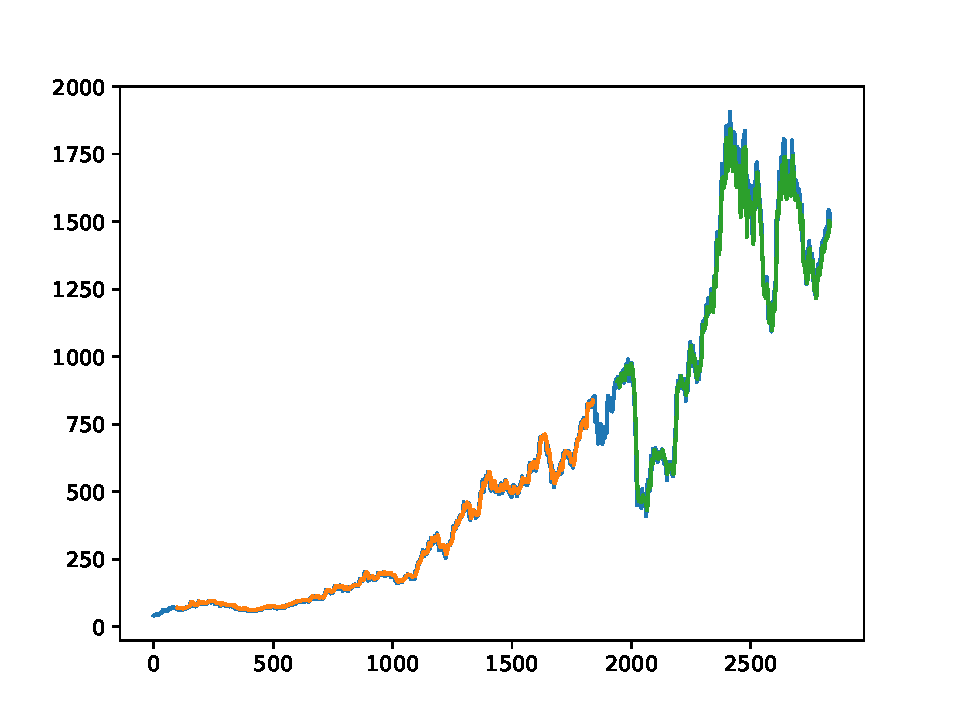
\includegraphics[scale=.65]{output-files/lstm/test-train.pdf}
    \caption{Train-test fit}
    \label{fig:enter-label}\par}
\end{figure}
\pagebreak
\noindent When the model was used to predict the stock price for the next 30 days, the following plot was obtained-
\begin{figure}[H]
    \centering
    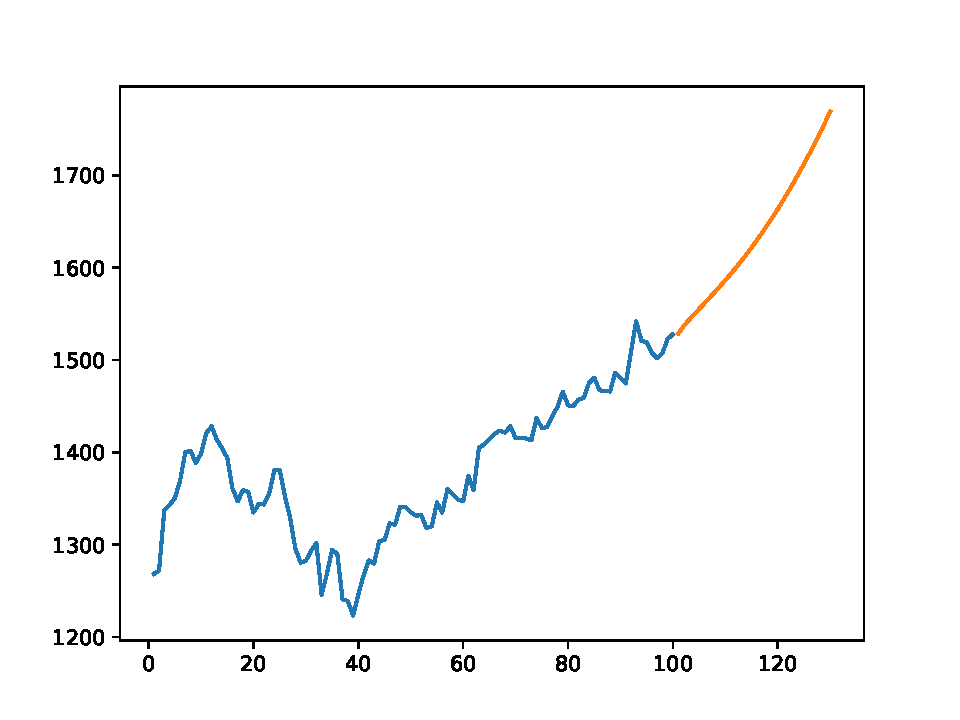
\includegraphics[scale=.75]{output-files/lstm/30dayprediction.pdf}
    \caption{30 day price prediction using stacked LSTM Model}
    \label{fig:enter-label}
\end{figure}
\subsection{XGBoost Model}
\begin{center}
    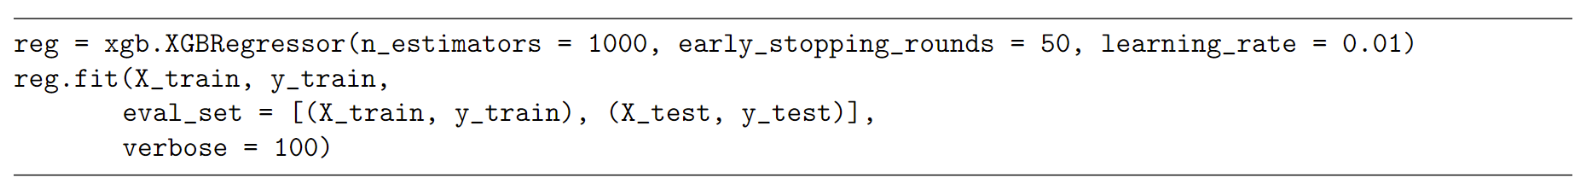
\includegraphics[scale=0.58]{codes/code 3.png}
\end{center}
% \begin{lstlisting}
% reg = xgb.XGBRegressor(n_estimators = 1000, early_stopping_rounds = 50, learning_rate = 0.01)
% reg.fit(X_train, y_train, 
%         eval_set = [(X_train, y_train), (X_test, y_test)], 
%         verbose = 100)
% \end{lstlisting}
This piece of code makes use of a model known as XGBoost, which is an abbreviation for "Extreme Gradient Boosting." XGBoost is a well-known method for machine learning that is praised for the effectiveness, adaptability, and excellent performance it offers. It belongs to the class of frameworks known as gradient boosters and was developed with the express purpose of maximizing both speed and performance. \cite{xgboost}

The XGBoost model uses machine learning techniques that are implemented with the assistance of parallel processing. As a result, it is both quicker and more effective than the conventional gradient boosting approaches. This is made possible by the fact that the loops that are used to form basic learners may be interchanged, which in turn makes parallel computing possible. Regularization is another feature that is included into XGBoost. This feature uses L1 (Lasso Regression) and L2 (Ridge Regression) in order to penalize complicated models and prevent overfitting. In addition to this, it includes built-in support for managing sparse data and missing values, and it employs a sparse-aware method to handle the various sparsity patterns that might be found in the data. The model also makes use of a one-of-a-kind tree pruning strategy, according to which the tree is allowed to grow to its maximum depth before beginning the pruning process, which continues in reverse until the amount of improvement in the loss function falls below a predetermined threshold.\\ 
The data was split into trian and test at 2018-05-04 as follows - 
\begin{figure}[H]
    \centering
    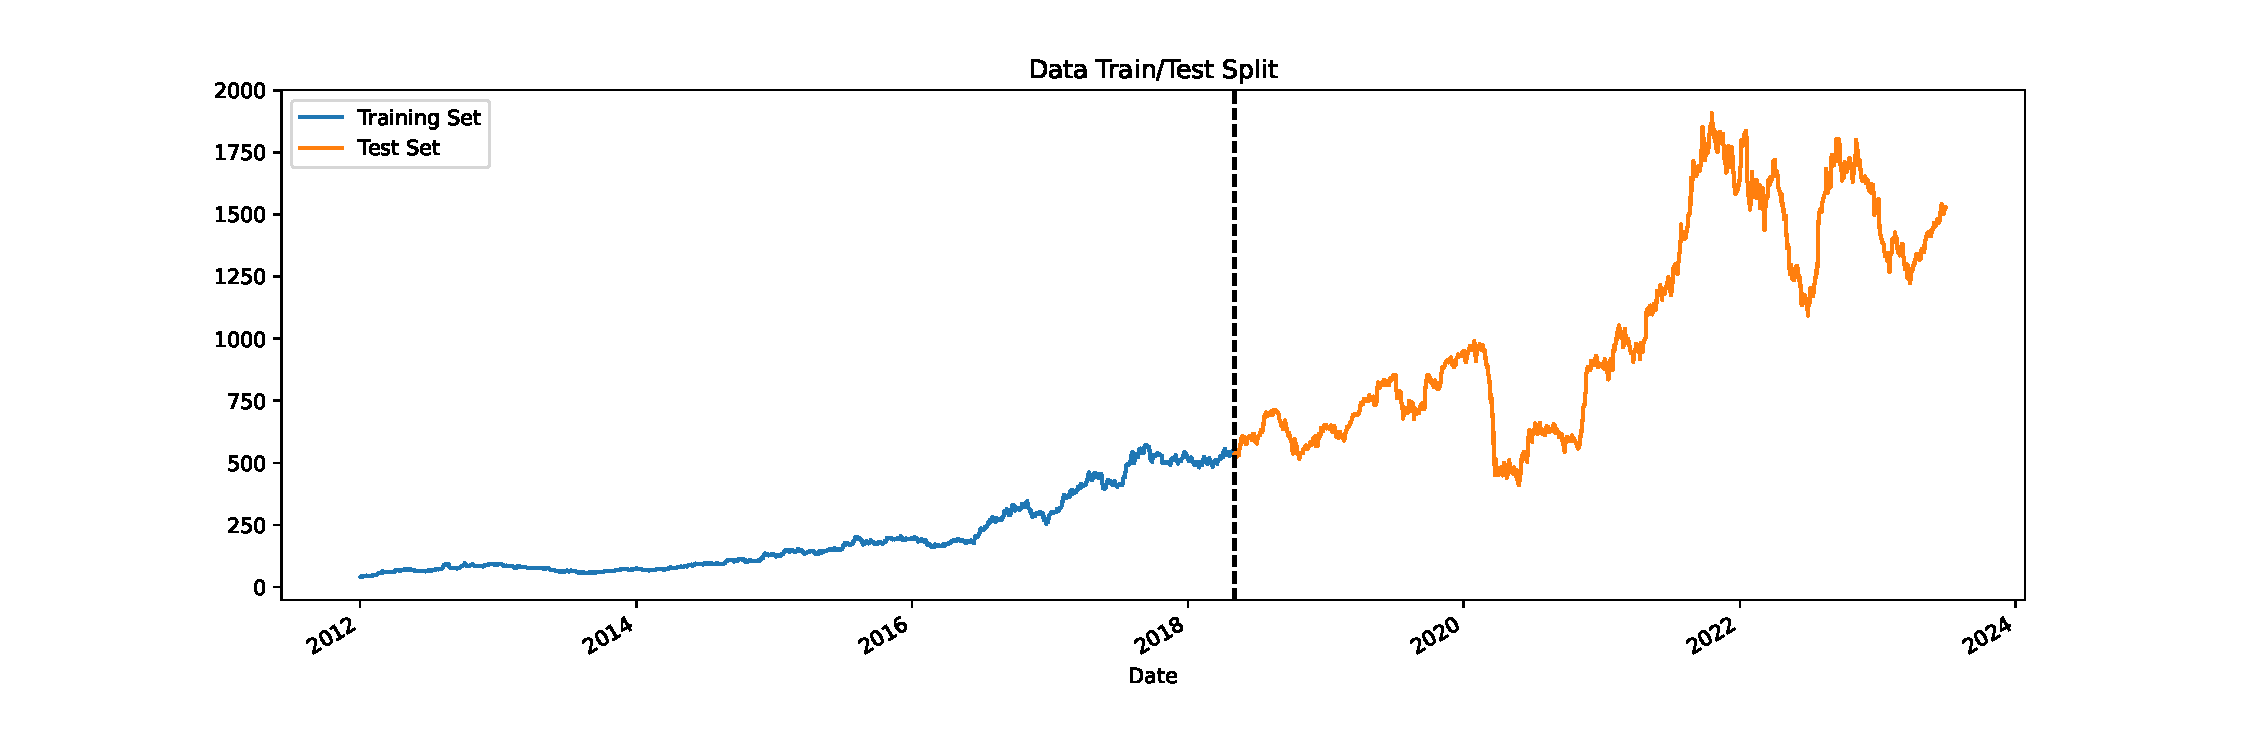
\includegraphics[scale=.5]{output-files/xgb/Test-train split.pdf}
    \caption{Test-train split}
    \label{fig:enter-label}
\end{figure}
In addition, XGBoost has built-in cross-validation at each iteration of the boosting process. As a result, it is much simpler to determine the precise ideal number of boosting rounds for a single run of the algorithm. In addition to this, it offers ongoing training, which enables you to train an initial model even further. 
\begin{center}
    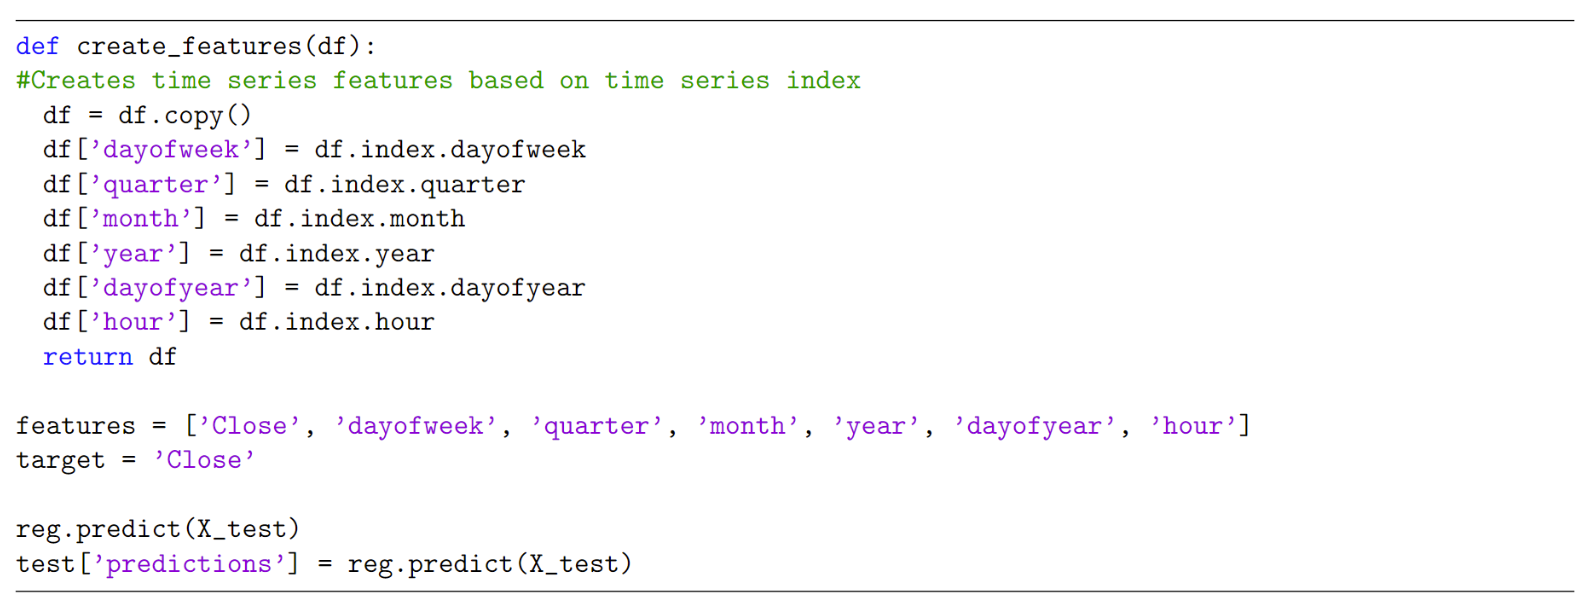
\includegraphics[scale=0.59]{codes/code 4.png}
\end{center}
% \begin{lstlisting}
% def create_features(df):
% #Creates time series features based on time series index
%   df = df.copy()
%   df['dayofweek'] = df.index.dayofweek
%   df['quarter'] = df.index.quarter
%   df['month'] = df.index.month
%   df['year'] = df.index.year
%   df['dayofyear'] = df.index.dayofyear
%   df['hour'] = df.index.hour
%   return df

% features = ['Close', 'dayofweek', 'quarter', 'month', 'year', 'dayofyear', 'hour']
% target = 'Close'

% reg.predict(X_test)
% test['predictions'] = reg.predict(X_test)
% \end{lstlisting}
\noindent The XGBoost model in this piece of code makes use of time series characteristics such the day of the week, quarter, month, year, and day of the year, in addition to lag features that reflect data from earlier time periods.
\pagebreak
\\ Here, is a plot showing the predictions from XGBoost Model-
\vspace{0.1in}
\hrule
\begin{center}
    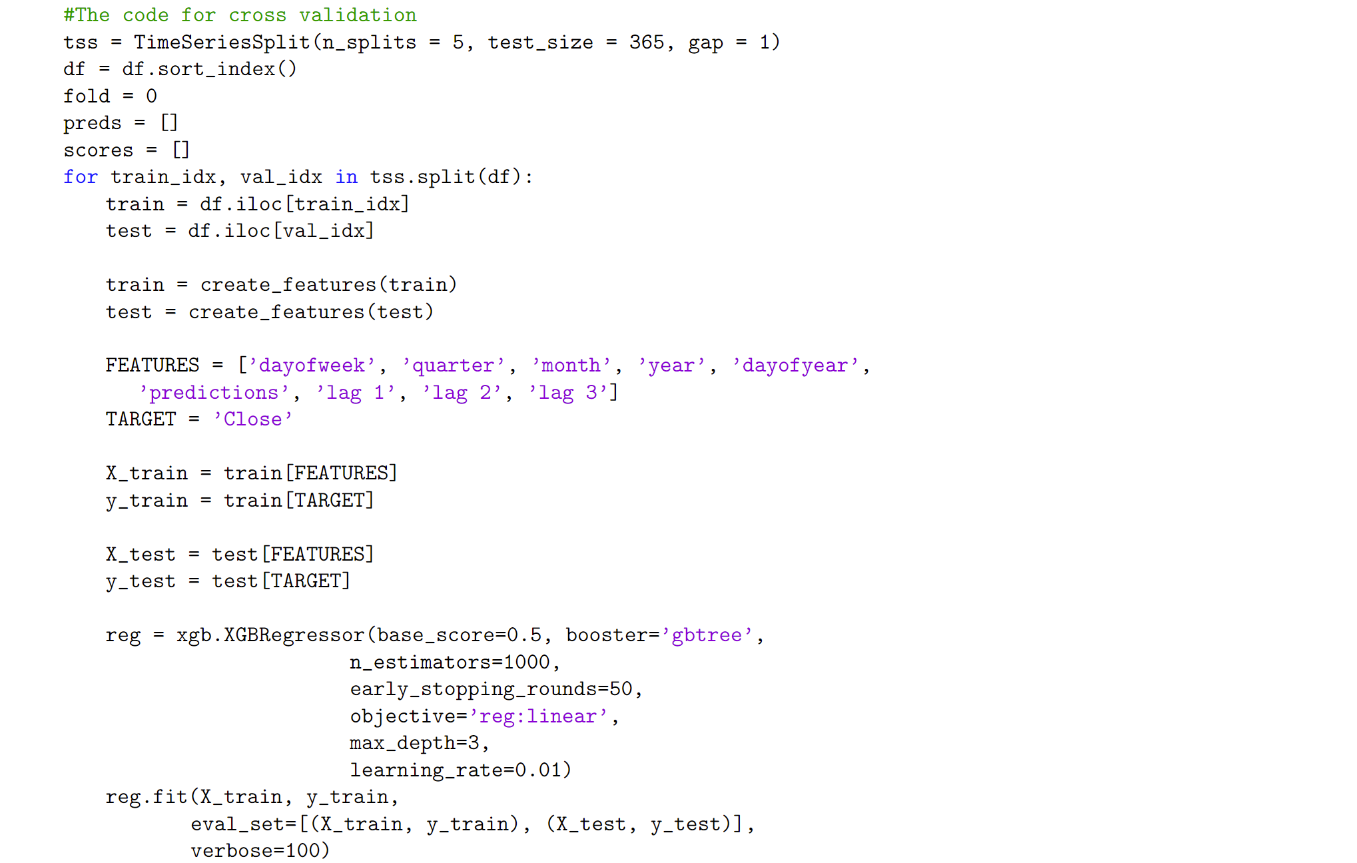
\includegraphics[scale=0.59]{codes/code 5.png}
\end{center}
\hrule
\vspace{0.1in}
% \begin{lstlisting}
% #The code for cross validation
% tss = TimeSeriesSplit(n_splits = 5, test_size = 365, gap = 1)
% df = df.sort_index()
% fold = 0
% preds = []
% scores = []
% for train_idx, val_idx in tss.split(df):
%     train = df.iloc[train_idx]
%     test = df.iloc[val_idx]

%     train = create_features(train)
%     test = create_features(test)

%     FEATURES = ['dayofweek', 'quarter', 'month', 'year', 'dayofyear',
%        'predictions', 'lag 1', 'lag 2', 'lag 3']
%     TARGET = 'Close'

%     X_train = train[FEATURES]
%     y_train = train[TARGET]

%     X_test = test[FEATURES]
%     y_test = test[TARGET]

%     reg = xgb.XGBRegressor(base_score=0.5, booster='gbtree',
%                            n_estimators=1000,
%                            early_stopping_rounds=50,
%                            objective='reg:linear',
%                            max_depth=3,
%                            learning_rate=0.01)
%     reg.fit(X_train, y_train,
%             eval_set=[(X_train, y_train), (X_test, y_test)],
%             verbose=100)
% \end{lstlisting}
After that, the model is tested for its resilience by being cross-validated over a variety of time periods. The final model is used to create predictions based on data that will be collected in the future.
\begin{center}
    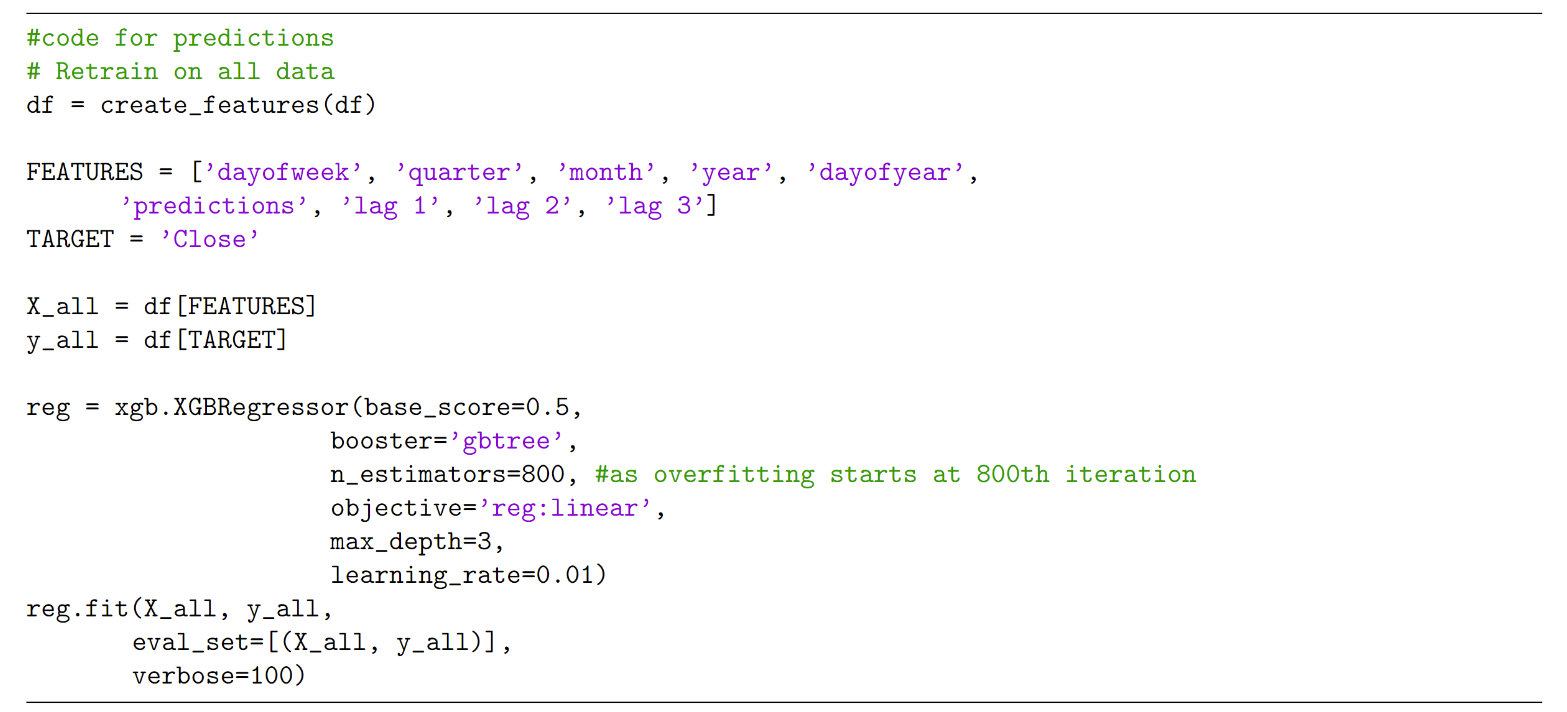
\includegraphics[scale=0.5]{codes/code 6.png}
\end{center}
% \begin{lstlisting}
% #code for predictions
% # Retrain on all data
% df = create_features(df)

% FEATURES = ['dayofweek', 'quarter', 'month', 'year', 'dayofyear',
%        'predictions', 'lag 1', 'lag 2', 'lag 3']
% TARGET = 'Close'

% X_all = df[FEATURES]
% y_all = df[TARGET]

% reg = xgb.XGBRegressor(base_score=0.5,
%                        booster='gbtree',
%                        n_estimators=800, #as overfitting starts at 800th iteration
%                        objective='reg:linear',
%                        max_depth=3,
%                        learning_rate=0.01)
% reg.fit(X_all, y_all,
%         eval_set=[(X_all, y_all)],
%         verbose=100)
% \end{lstlisting}
\pagebreak

The predictions from our model look like the following when plotted-
\begin{figure}[H]
    \centering
    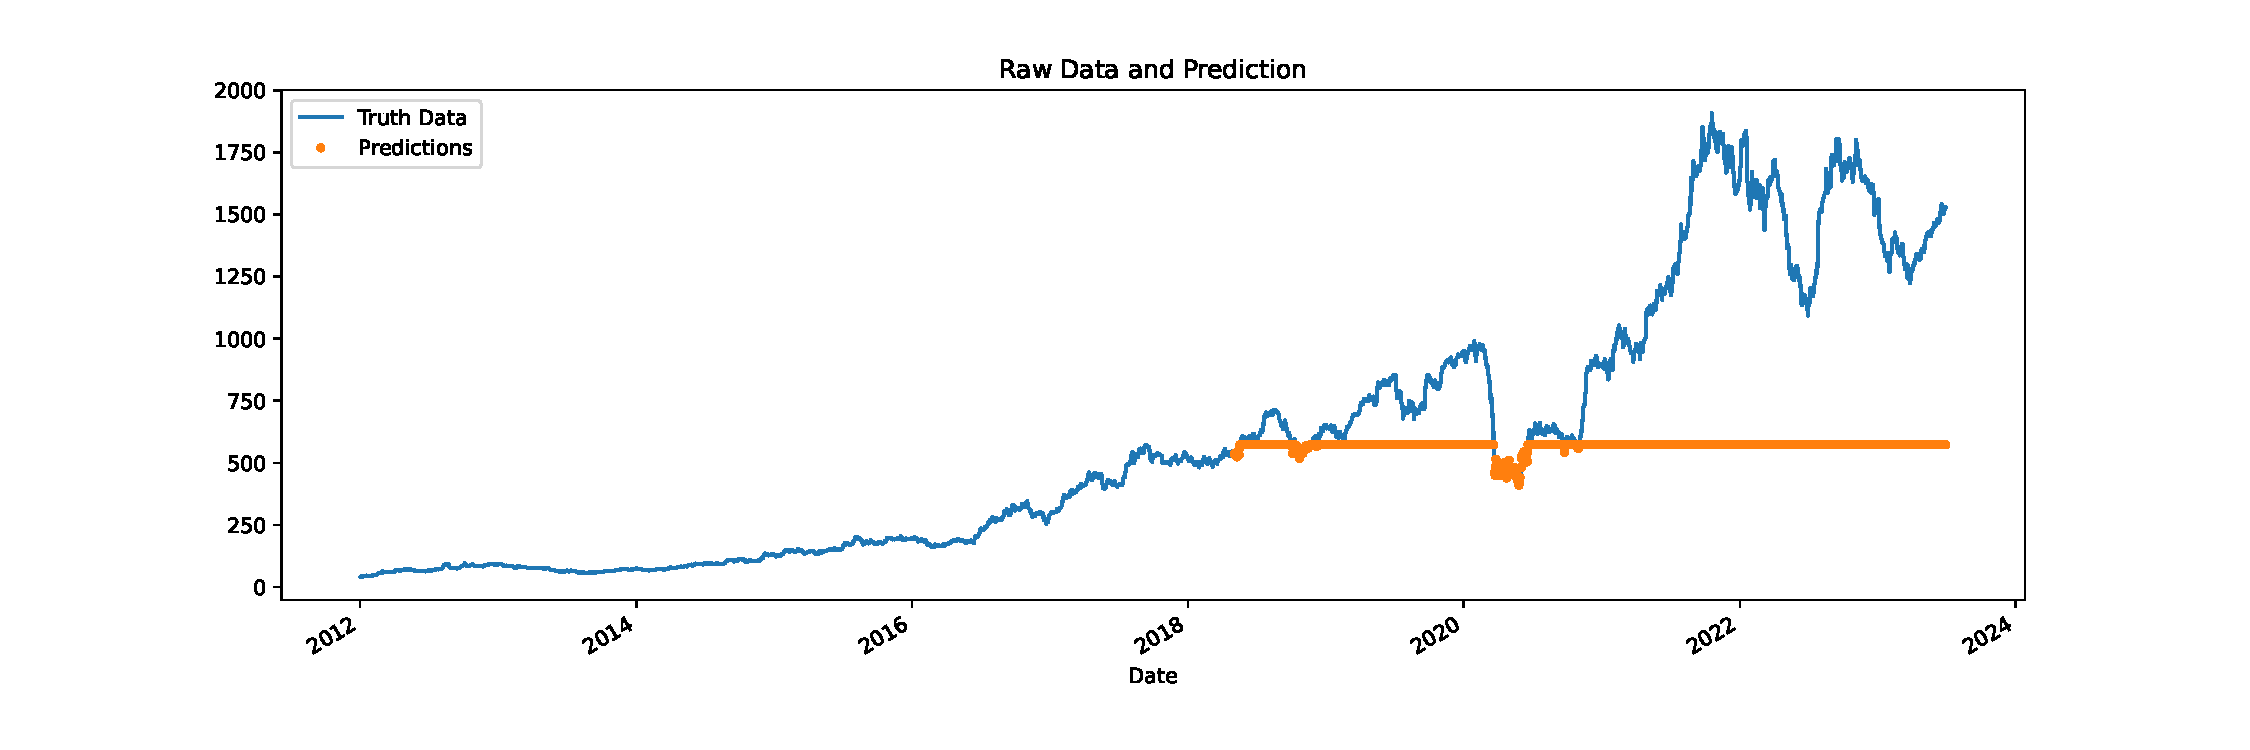
\includegraphics[scale=.5]{output-files/xgb/raw-data-pred.pdf}
    \caption{Predicitions while training and testing}
    \label{fig:enter-label}
\end{figure}
\begin{figure}[H]
    \centering
    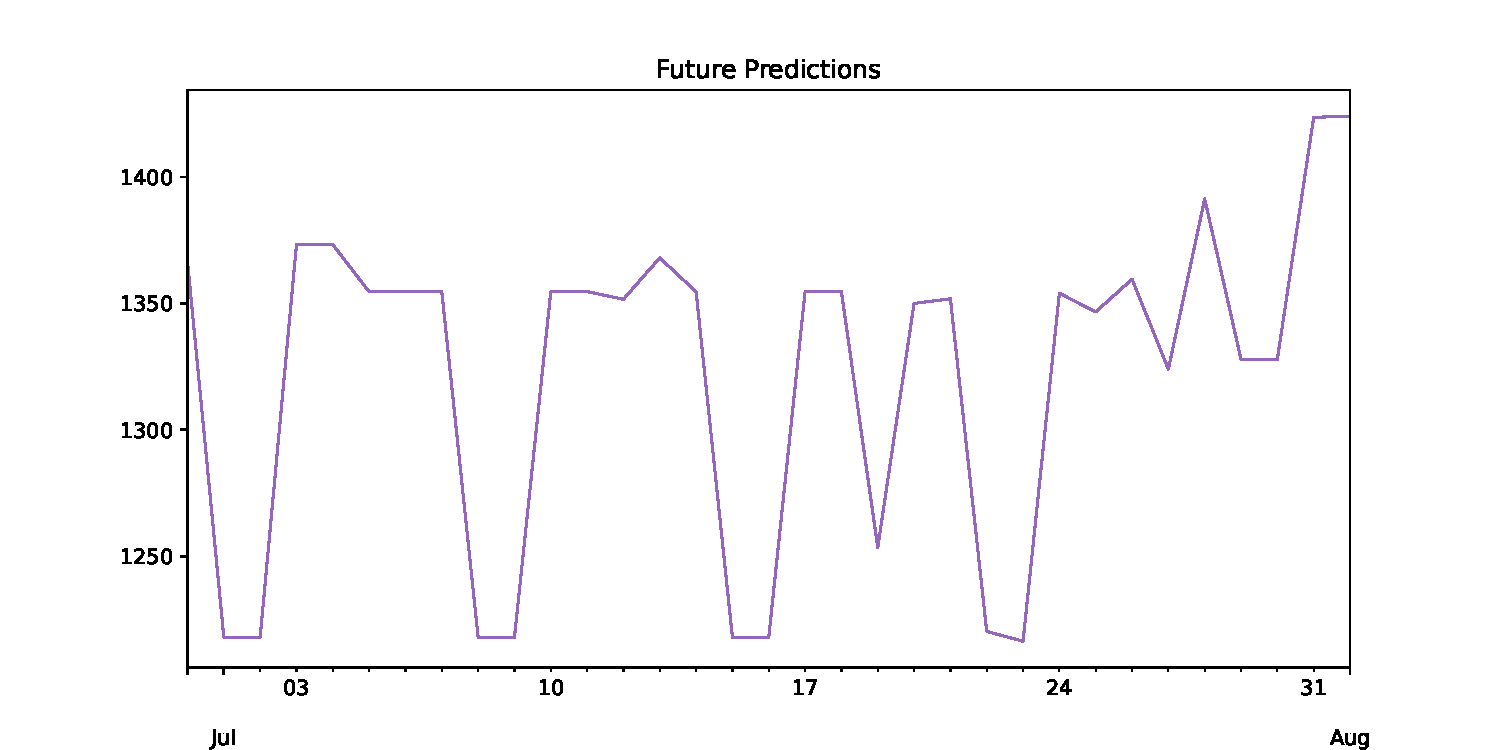
\includegraphics[scale=.75]{output-files/xgb/future-pred.pdf}
    \caption{Future Predictions}
    \label{fig:enter-label}
\end{figure}
\subsection{FBProphet Model}
Prophet, a forecasting tool developed by Facebook, is employed in this architecture. Prophet is a piecewise linear or logistic growth curve trending additive regression model. \cite{fbprophet} It has an annual seasonal component that is modeled using Fourier series and a weekly seasonal component that is modeled using dummy variables. \cite{fbprophetpaper}

The model uses Pandas for data manipulation, matplotlib and seaborn for data visualization, Prophet for forecasting, and sklearn for performance measurements are among the tools available. 

The data was read from a CSV file and any null values are deleted. The data was then visualized using matplotlib to have a better understanding of the time-series distribution. 
\begin{figure}[H]
    \centering
    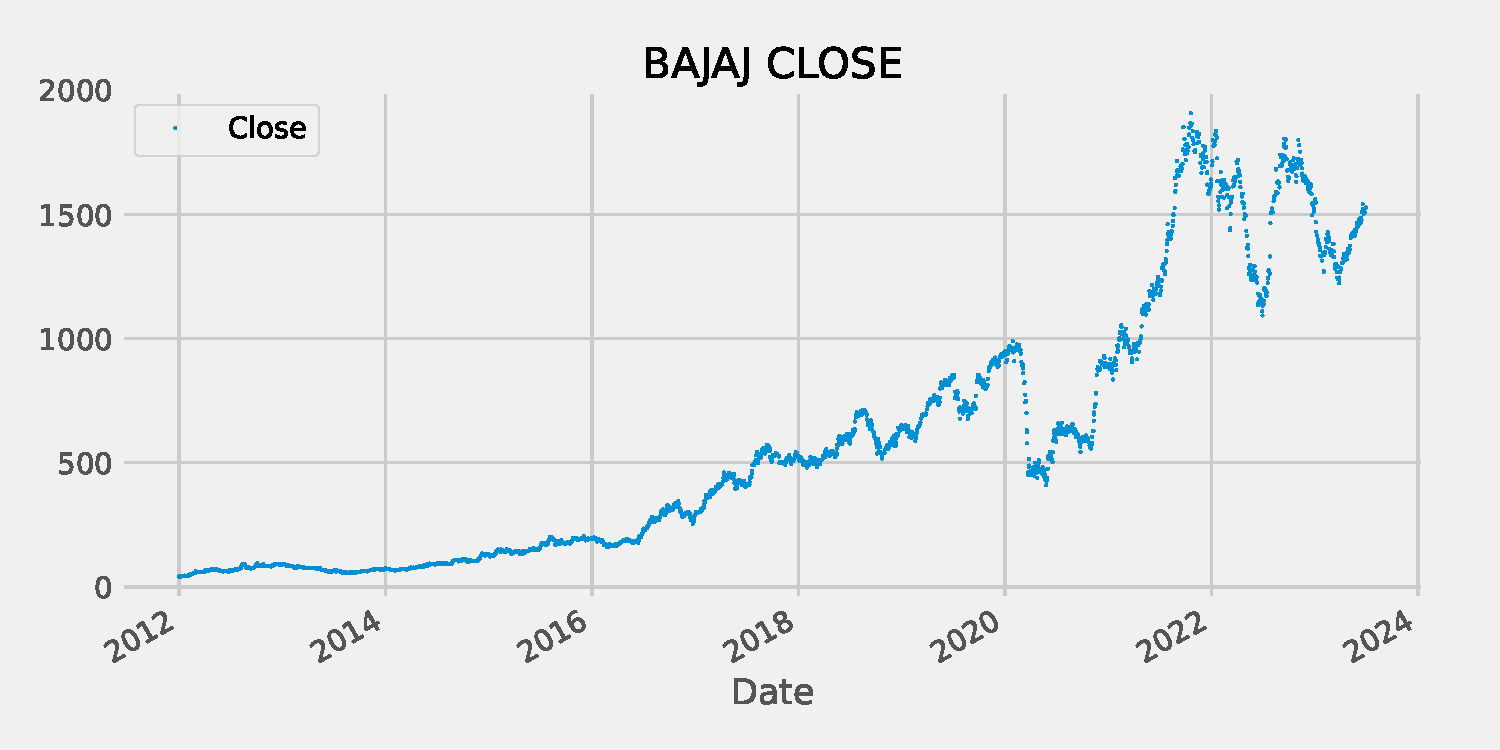
\includegraphics[scale=0.5]{output-files/fbprophet/data (1).pdf}
    \caption{Data used in the model}
    \label{fig:enter-label}
\end{figure}
The data was prepared such that it was compatible with the Prophet. Prophet expects data in a specified format, with two columns: 'ds' for date-time and 'y' for the variable to predict.
\vspace{-0.2in}
\begin{center}
    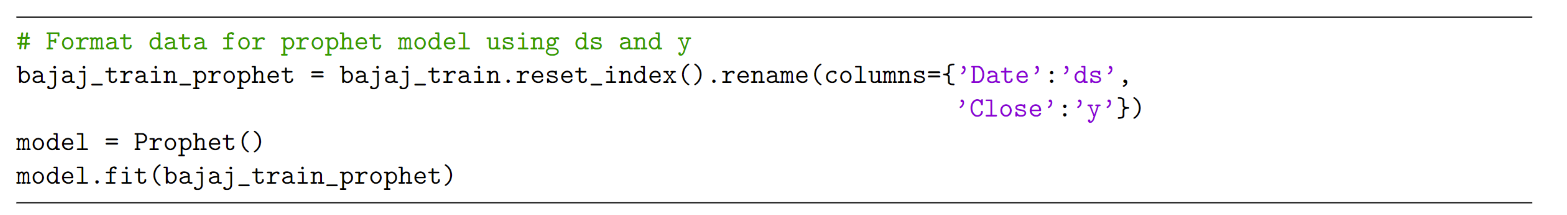
\includegraphics[scale=0.59]{codes/code 7.png}
\end{center}
% \begin{lstlisting}
% # Format data for prophet model using ds and y
% bajaj_train_prophet = bajaj_train.reset_index().rename(columns={'Date':'ds',
%                                                                        'Close':'y'})
% model = Prophet()
% model.fit(bajaj_train_prophet)
% \end{lstlisting}    
\noindent The data was then split into train-test as can be seen from the following graph-
\begin{figure}[H]
    \centering
    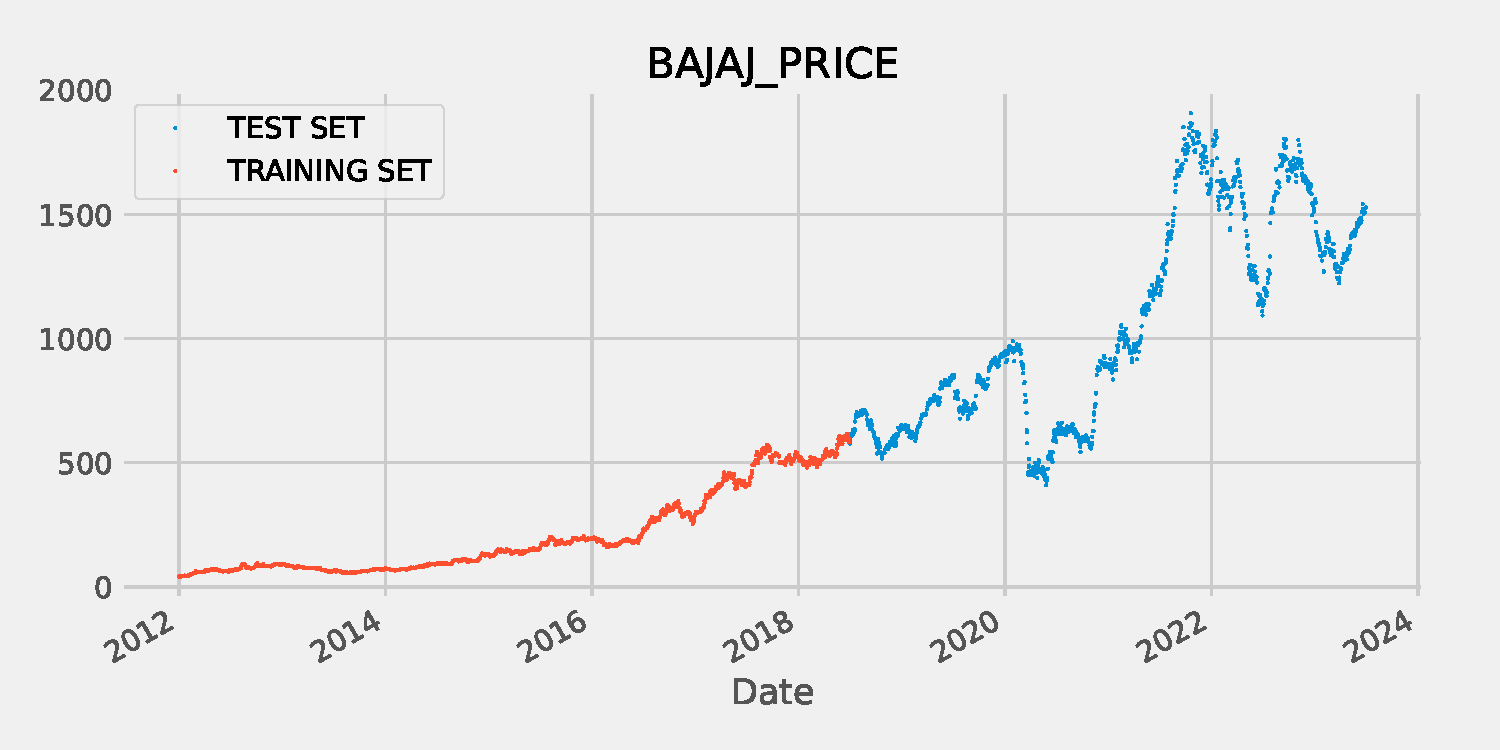
\includegraphics[scale=0.45]{output-files/fbprophet/split (1).pdf}
    \caption{Train-test split}
    \label{fig:enter-label}
\end{figure}

A Prophet model was created and fitted to the training data. The model was used to forecast stock values based on test data.

\noindent The plot of the same be seen as follows - 
\vspace{-.1in}
\begin{figure}[H]
    \centering
    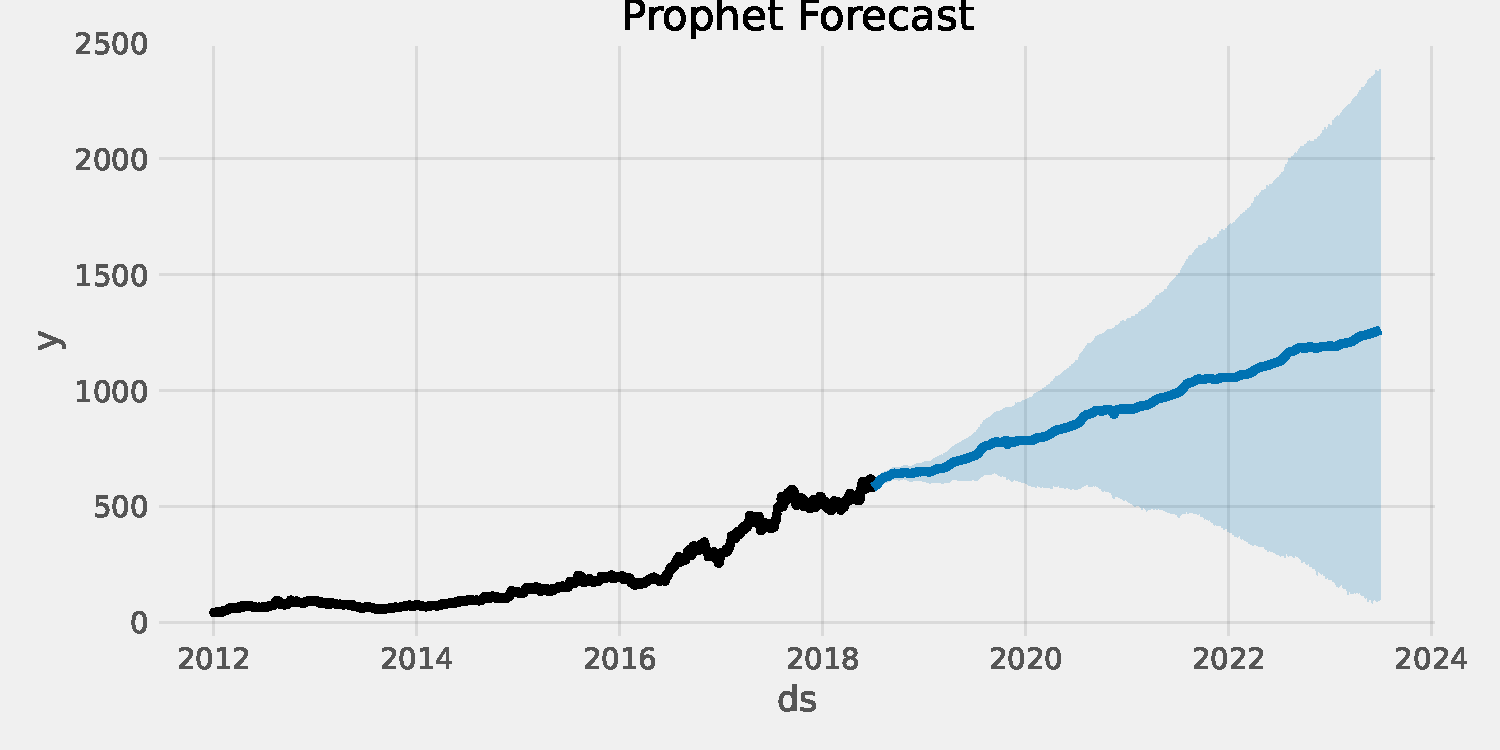
\includegraphics[scale=0.53]{output-files/fbprophet/forecast (1).pdf}
    \caption{Forecast given by FBProphet model}
    \label{fig:enter-label}
\end{figure}

\noindent The forecast was then visualized and assessed using root mean squared error (RMSE), mean absolute error (MAE), and mean absolute percentage error (MAPE). Finally, a future dataframe was generated to provide forecasts for the following 365 days.
\begin{center}
    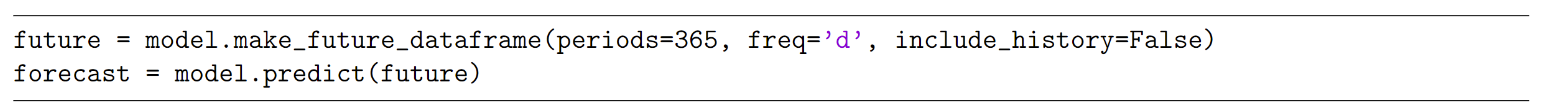
\includegraphics[scale=0.59]{codes/code 8.png}
\end{center}
% \begin{lstlisting}
% future = model.make_future_dataframe(periods=365, freq='d', include_history=False)
% forecast = model.predict(future)
% \end{lstlisting}
The output obtained is the following - \\
\begin{center}
\begin{varwidth}{\linewidth}
\begin{verbatim}
            ds        yhat
0   2018-06-30  568.392435
1   2018-07-01  568.857409
2   2018-07-02  583.428675
3   2018-07-03  584.257763
4   2018-07-04  584.839007

\end{verbatim}
\end{varwidth}
\end{center}
\pagebreak
\noindent The comparison of the predictions made by the model and the actual test values can been from the following \\plot -
\begin{figure}[H]
    \centering
    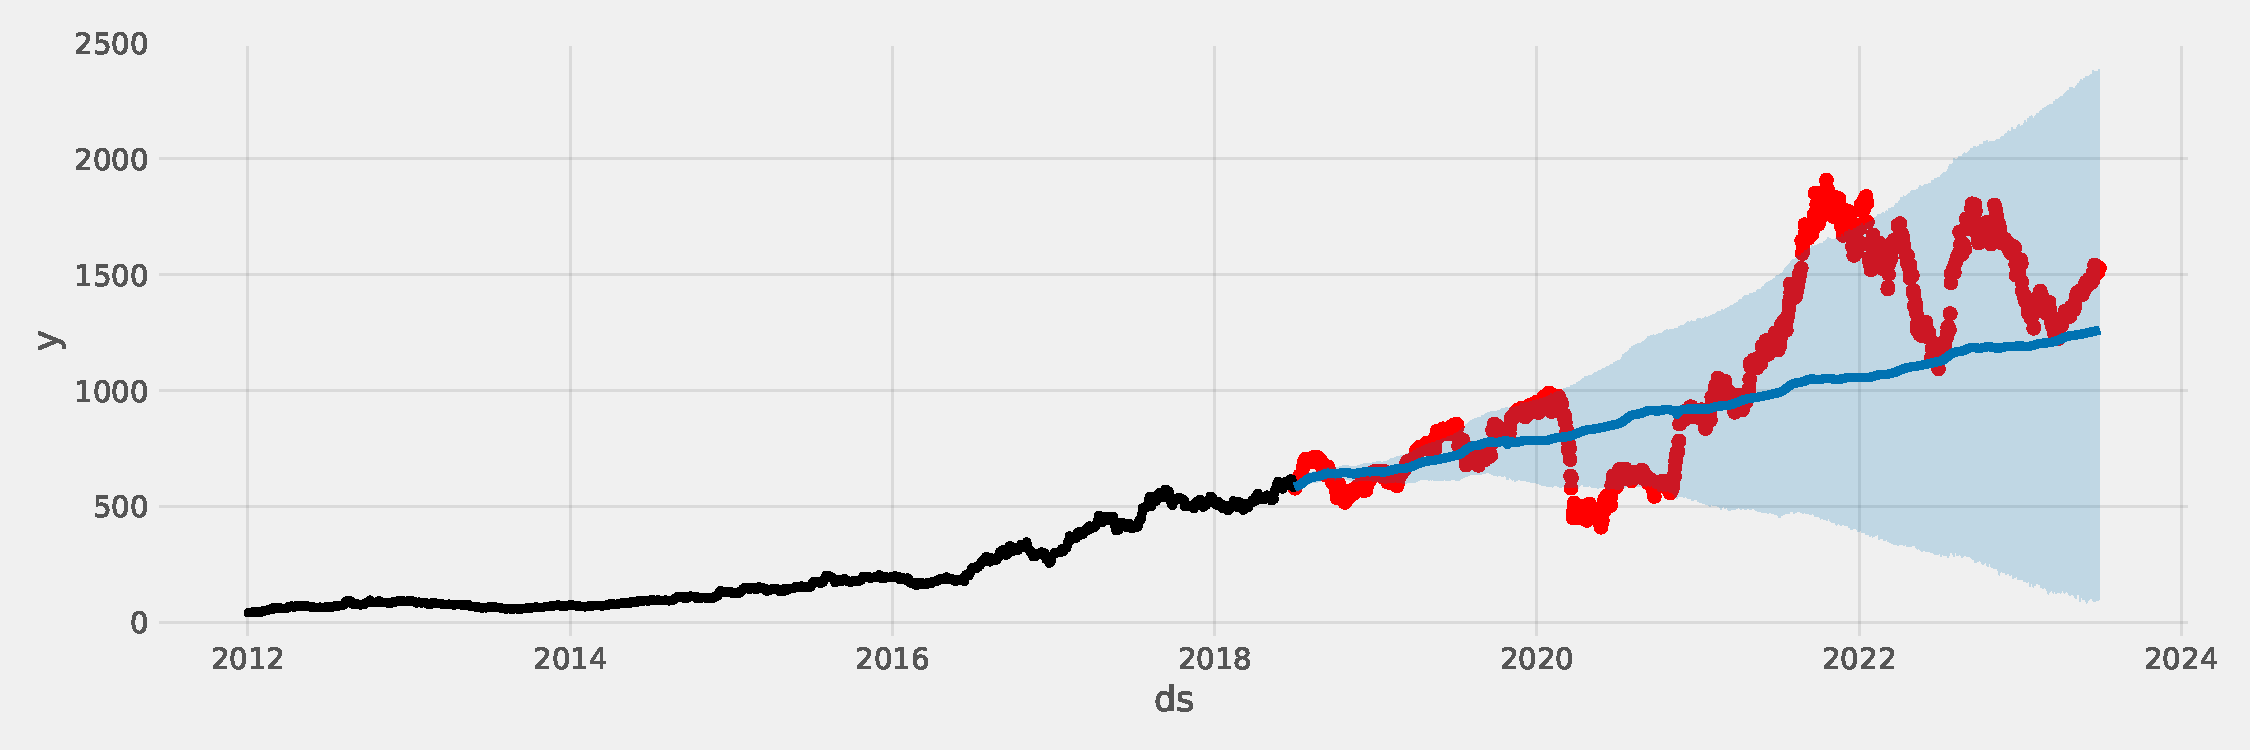
\includegraphics[scale=0.5]{output-files/fbprophet/comparison.pdf}
    \caption{Actual values v/s Predicted values}
    \label{fig:enter-label}
\end{figure}
\section{Evaluation}
\subsection{Metrics}
The metric which was used to compare the models was \textbf{mean absolute percentage error (MAPE).}\\ {The function for calculating the MAPE was defined as follows - }
\begin{center}
    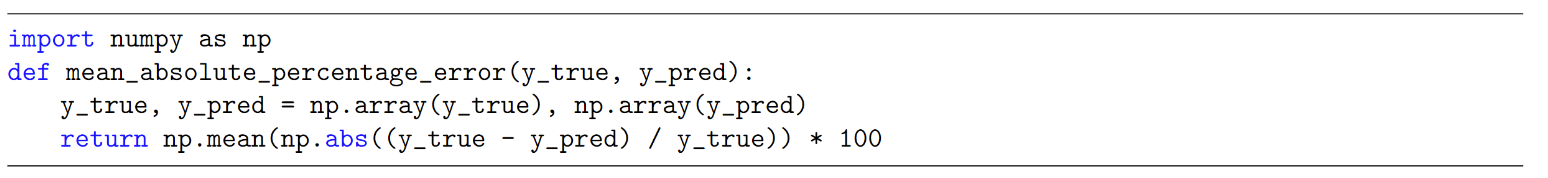
\includegraphics[scale=0.6]{codes/code 9.png}
\end{center}
% \begin{lstlisting}
% import numpy as np
% def mean_absolute_percentage_error(y_true, y_pred):
%     y_true, y_pred = np.array(y_true), np.array(y_pred)
%     return np.mean(np.abs((y_true - y_pred) / y_true)) * 100
% \end{lstlisting}
\subsection{Comparison}
On comparing the models based on their MAPE values, it was found that the FBProphet model outperforms both LSTM and XGBoost models. LSTM model showed a really low accuracy and hence, a poor performance and isn't recommended for forecasting models. 
\pagebreak

The comparison of the models on the basis on MAPE can be seen in the following table -
\begin{table}[h]
\begin{adjustbox}{width=\columnwidth-2.5in,center}
    \centering
\begin{tabular}{@{}llll@{}}
\toprule
\textbf{Model} & \textbf{LSTM Model} & \textbf{XGBoost Model} & \textbf{FBProphet Model} \\ \midrule
\textbf{MAPE}  & 235135\%            & 36.67\%                & 21.53\%                  \\ \bottomrule
\end{tabular}
\end{adjustbox}
\caption{Comparison of the models}
\end{table}
\section{Conclusion}
In conclusion, this research project explored the application of advanced machine learning models such as Stacked LSTMs, XGBoost, and Facebook's Prophet Model to predict the stock price of Bajaj Finserv for the next 30 days using a 10-year data set of closing prices. These models were chosen based on their robustness and prior successful utilization in the field of stock price prediction.

The data was prepared meticulously by scaling it between 0 and 1 and implementing a train-test split strategy with a time-step of 100 days. This process ensured that the models were trained and tested on a comprehensive and varied dataset. The LSTM model consisted of three layers and a dense layer, trained on 100 epochs using the Adam optimizer. The model's performance was evaluated using RMSE and MAPE metrics. In parallel, we utilized Facebook's Prophet model, incorporating annual and weekly seasonal components, and XGBoost, a high-performing, gradient-boosting model with parallel processing and regularization capabilities.

The outcomes of this research can provide invaluable assistance to a range of stakeholders, including portfolio managers, risk management experts, and financial regulators. By using these predictive models, these individuals and groups can make well-informed decisions, reducing risk and maximizing returns. However, it is worth mentioning that these models, despite their robustness, are not without limitations, such as computational intensity and sensitivity to hyperparameter selection.

Overall, this study demonstrates that machine learning models hold significant potential in predicting stock prices, thereby assisting in strategic decision-making and risk management. This research contributes to the ongoing exploration and innovation in financial technology, demonstrating how advanced technology can be leveraged to predict market movements, thus enhancing financial stability and investor confidence. Future work could further refine these models and explore their application in different market scenarios and for various other stocks, potentially even in real-time prediction systems. This could revolutionize how one approaches stock trading and investment strategies, bringing about more precision, confidence, and profitability in financial markets.

\section{Acknowledgements}
We would like to extend our heartfelt appreciation to Dr. Aneesh Chivukula for his invaluable guidance and support throughout our work on the project titled "AI-Driven Stock Price Forecasting." Under his mentorship, we have gained a comprehensive understanding of stacked LSTM, XGBoost, and FBProphet models, and their application in the realm of stock market analysis. Dr. Aneesh's astute insights and unwavering support have enabled us to develop an accurate and efficient forecasting model, while his expertise in deep learning and data analysis has significantly enhanced our knowledge and skills in this fascinating field. We are sincerely grateful for the remarkable opportunity he has provided us, which has enriched our learning experience and paved the way for our success in AI-driven stock price forecasting.
\addcontentsline{toc}{section}{References}
\printbibliography
\end{document}